%          spconf.sty  - ICASSP/ICIP LaTeX style file, and
%          IEEEbib.bst - IEEE bibliography style file.
% --------------------------------------------------------------------------
\documentclass{article}
\usepackage{spconf,amsmath,graphicx}
\usepackage{booktabs}
\usepackage{hyperref}
\usepackage{caption}
\usepackage{float}


% Title.
% ------
\title{Resilient Security: Threat Modeling and Defensive Strategies for Large Language Models Platforms}
\name{SN: 24076607}
\address{}
%
\begin{document}

\maketitle
%
\begin{abstract}
    This report presents a comprehensive approach to securing Large Language Model (LLM) platforms through threat modeling and defensive strategy development. We analyze a Flask-based AI dialogue system with user authentication, conversation management, and content moderation capabilities. 
    Using STRIDE methodology, we identify and prioritize threats including session hijacking, brute force attacks, NoSQL injection, and DDoS attempts, demonstrating through practical simulations how adversaries could extract sensitive information. 
    We then implement a multi-layered defense incorporating MFA, bcrypt password hashing, rate limiting, HTTPS encryption, and AI-driven content filtering to prevent storing prohibited content. 
    The paper addresses regulatory compliance with GDPR, CRA, and PSTI frameworks while considering ethical implications of AI security systems. 
    Finally, we evaluate enterprise scaling considerations and innovative approaches like contextual authentication and privacy-preserving techniques to ensure long-term viability of secure LLM platforms.\footnote{The code is provided on GitHub: \url{https://github.com/yushiran/ELEC0138Coursework\_Group5}, and the presentation video is available at: \url{https://www.youtube.com/watch?v=0v1x2g4X8nE}.}
\end{abstract}
%
\begin{keywords}
    Large Language Models, threat modeling, cybersecurity, authentication, privacy, STRIDE, defensive strategies, ethical AI
\end{keywords}

\section{Coursework 1: Threat Modeling \& Attack Simulation}
\subsection{Introduction and objectives}
This project simulates a widely used AI dialogue model system developed using Flask (Python) and MongoDB, creating a user login, a registration interface and a LLM chat interface. The system stores the user account password and other related personal information in the MongoDB database, and the user's chat information is also stored in the associated database to protect and manage it. 
At the same time, machine learning is used to load the BERT model\cite{Devlin2019BERTPO} to identify and delete banned messages in the chat to prevent the database from being contaminated with banned messages.
The system will include the following elements, which will be analysed:
\begin{enumerate}
    \item Front-end HTML forms: login, registration, AI chat interface, etc.
    \item Back-end: a Flask-based server that manages user information and dialogue content.
    \item Database: MongoDB (local instance) to store user data and messages.
\end{enumerate}

First, when the webpage is opened, the interface is shown in the diagram below. Fig. \ref{fig:login} shows the system login interface and Fig. \ref{fig:registration} shows the registration interface that the system retrieves.
\begin{figure}[htb]
    \centering
    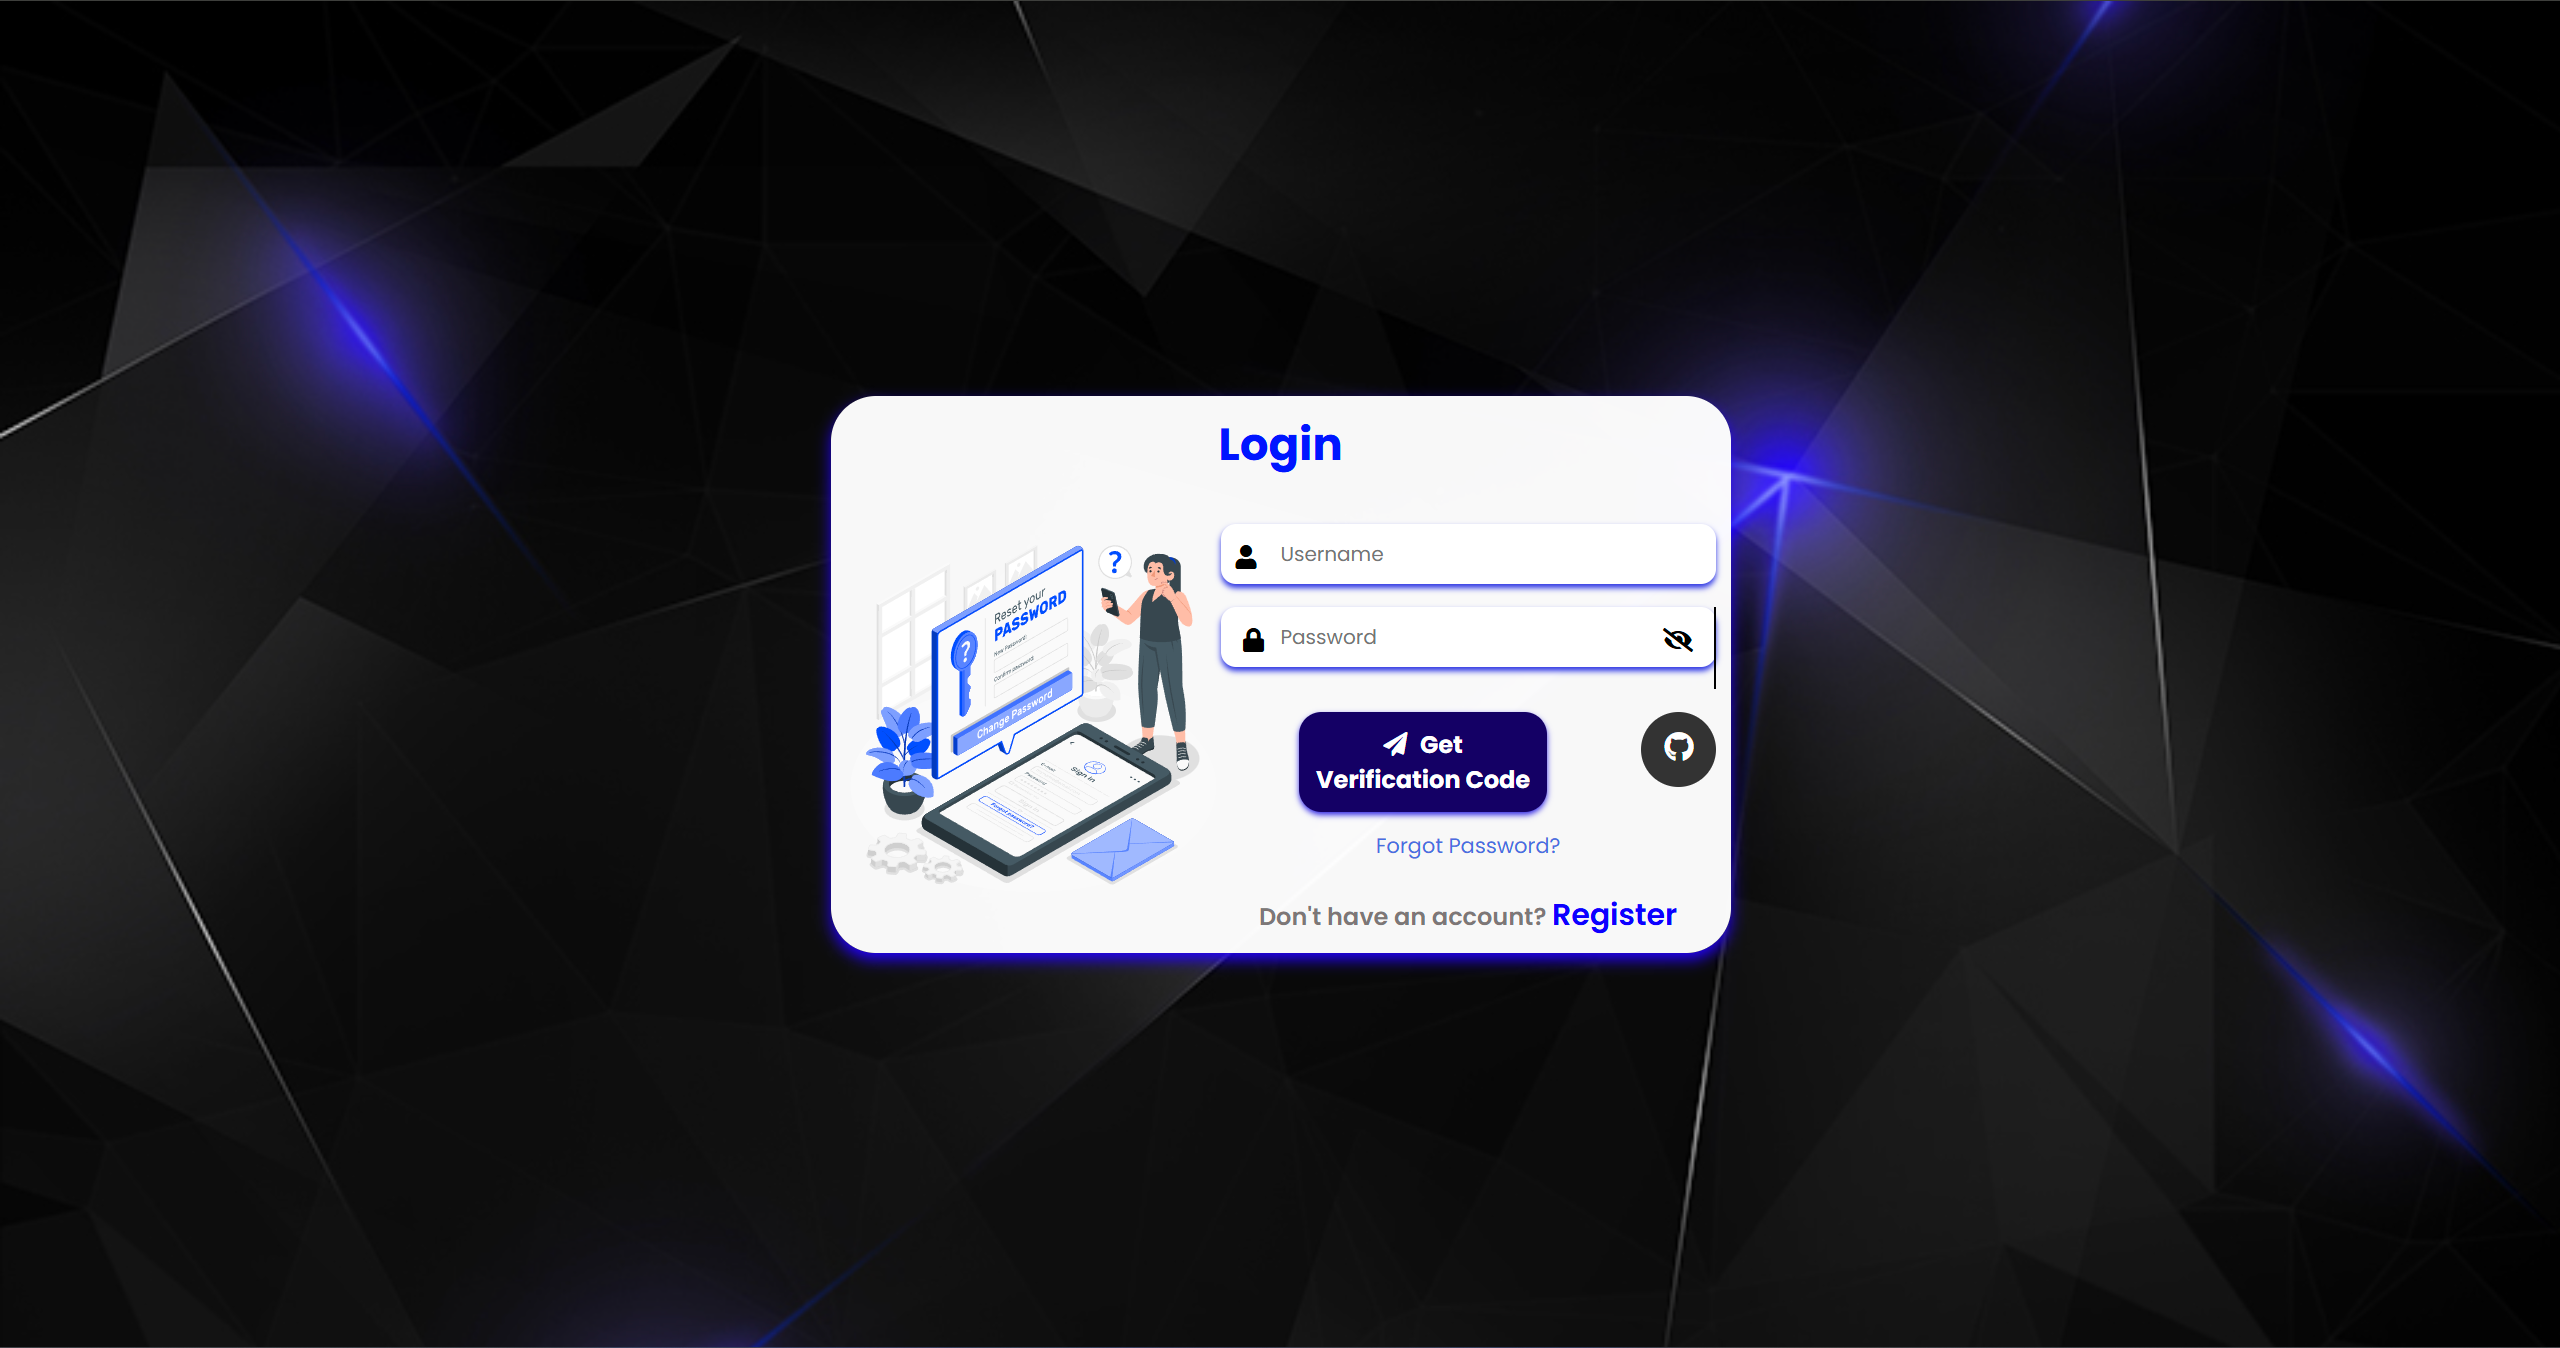
\includegraphics[width=0.5\textwidth]{images/login_screenshot.png}
    \caption{Login interface of the system}
    \label{fig:login}
\end{figure}

\begin{figure}[htb]
    \centering
    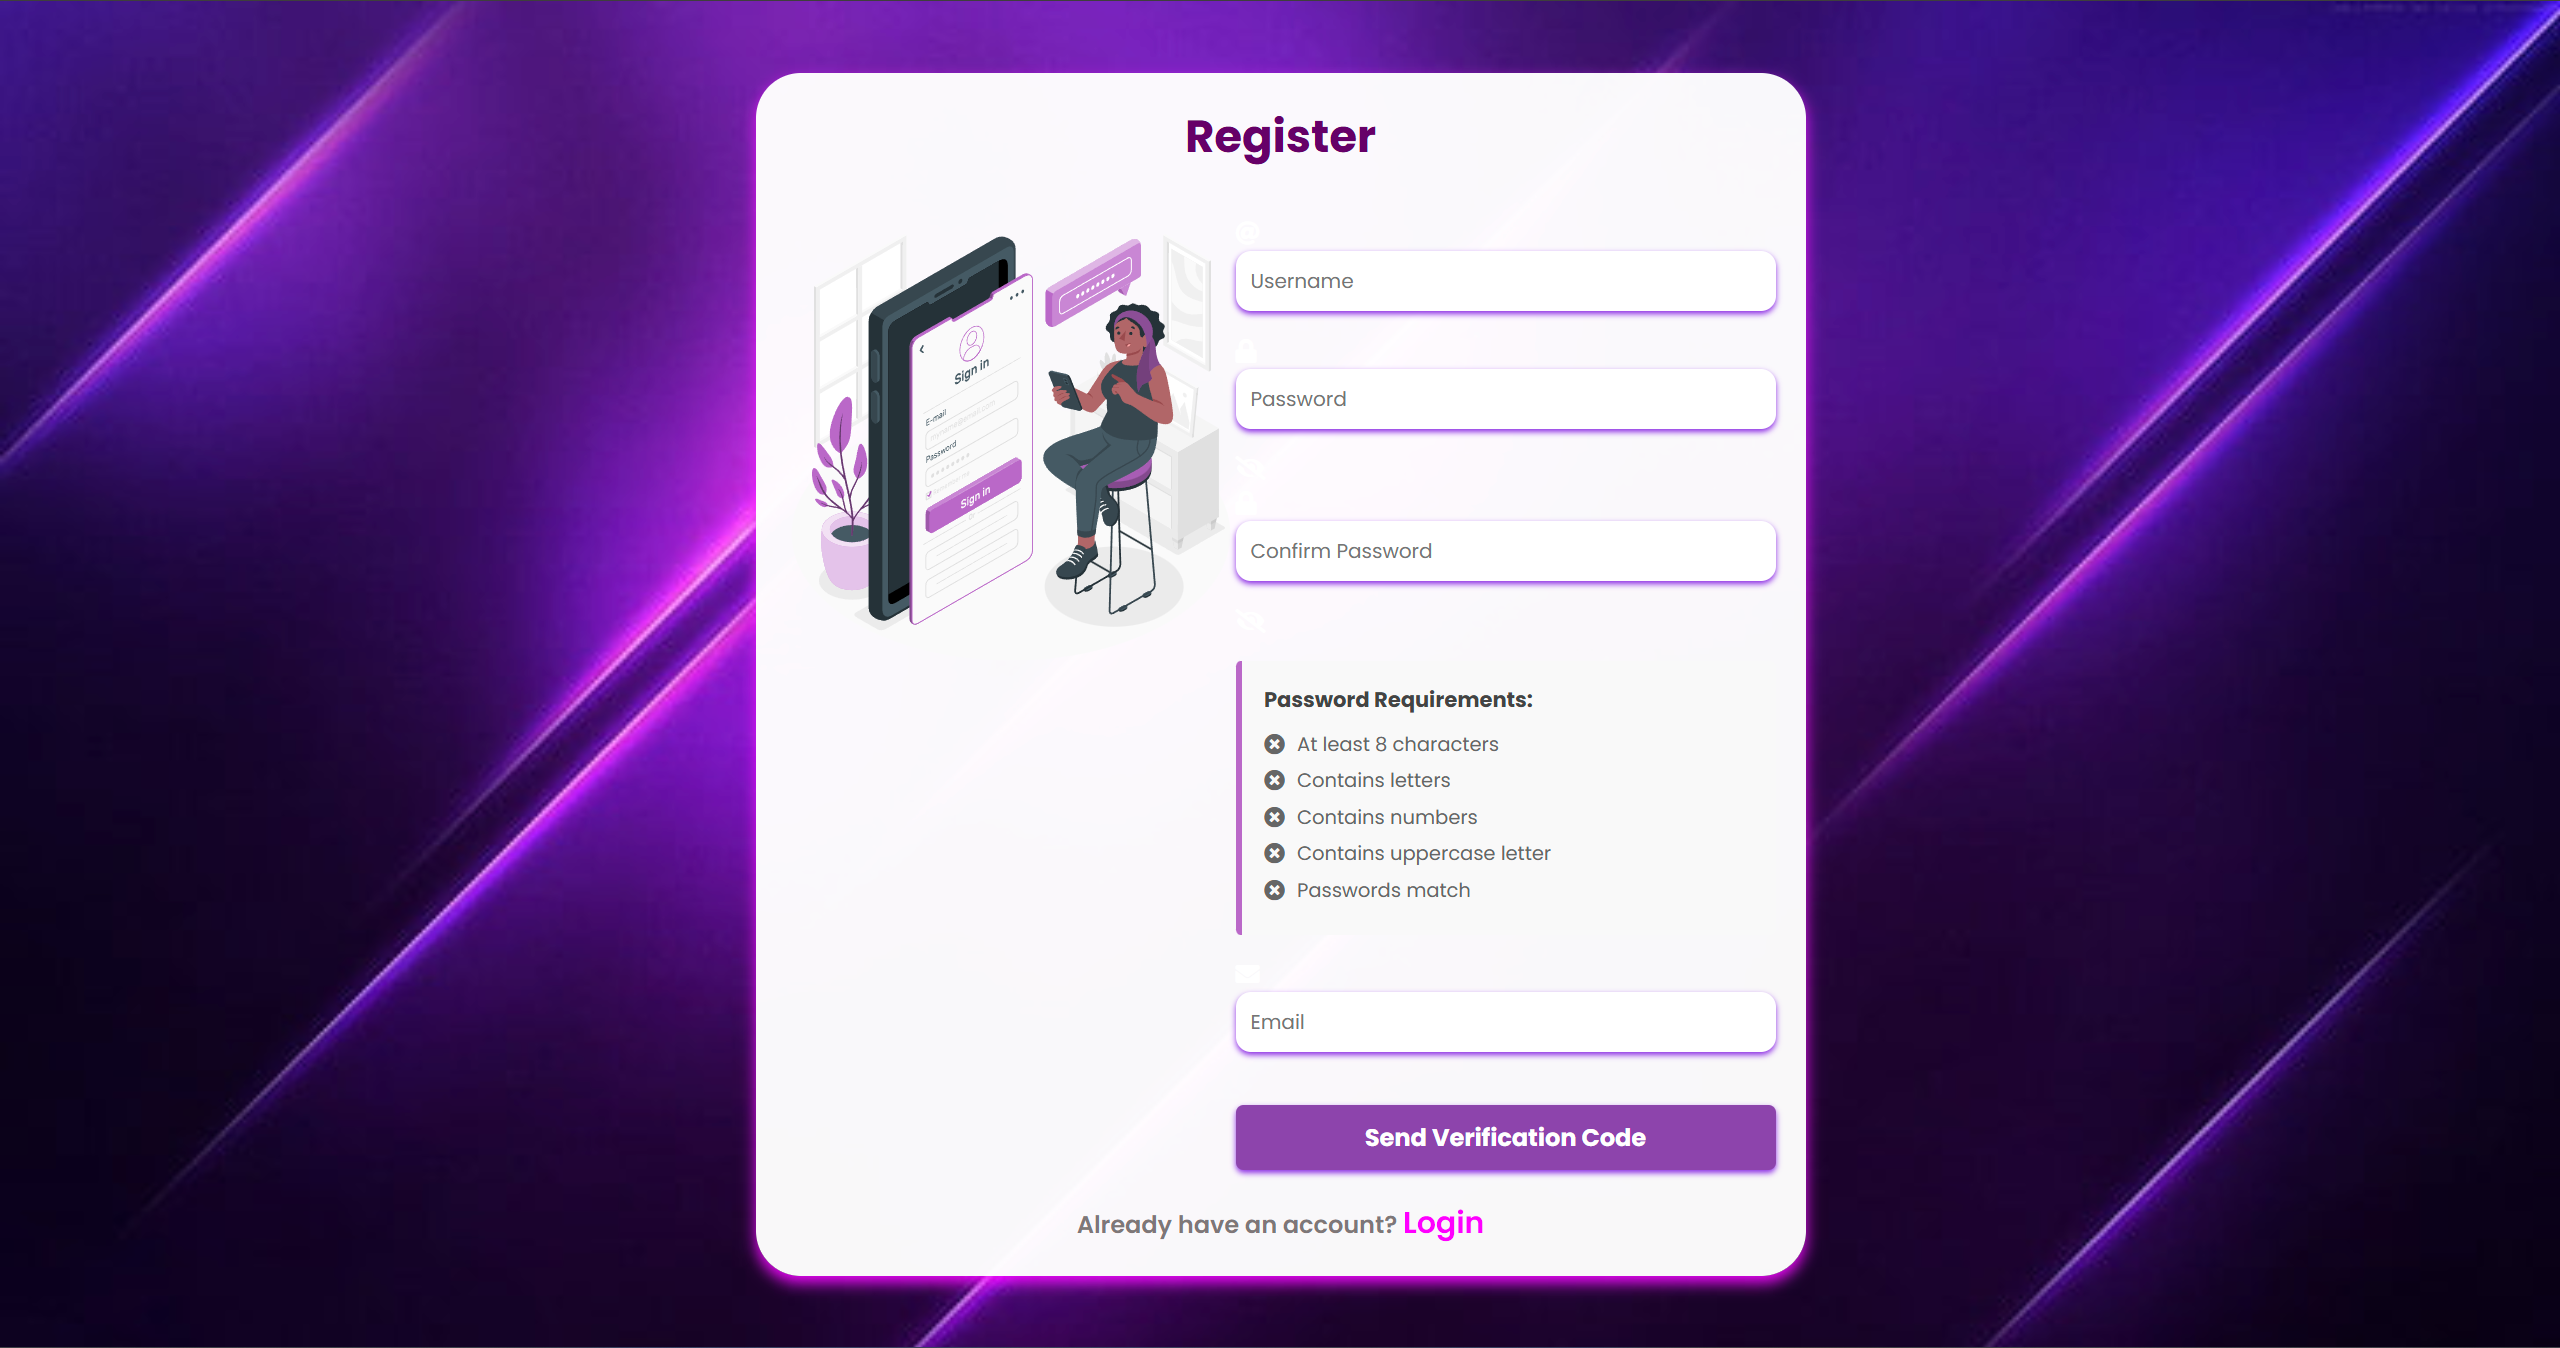
\includegraphics[width=0.5\textwidth]{images/registration_screenshot.png}
    \caption{Registration interface of the system}
    \label{fig:registration}
\end{figure}
After registration, a database message is generated in MongoDB containing all the user's personal data, including email address, password, etc. After logining, the user is redirected to the system's AI dialogue interface, where the same dialogue messages are machine-learned, classified and stored in the appropriate database.

There are several critical assets in the system and these are protected in the following to maintain privacy, data integrity and secure operation. The details are analysed below:

\begin{enumerate}
    \item user login and registration information: This information can be exposed when accessing web pages, submitting web pages, and in the MongoDB database, so if not stored in MongoDB using the bcrypt hash algorithm, successful intrusion by outsiders could lead to impersonation or unauthorized access.
    \item MongoDB databas: Data protection in the database is the most important part, which includes all legitimate personal data entered into the system. It also stores user conversations, including private data and illegal queries, which must be classified and monitored to avoid contamination of the local database.
    \item Session identifiers: This type of data is stored in client cookies across a Flask session and, if intercepted, a malicious user can access user data without logging in.
    \item System configuratio: System configuration information is unlikely to be exposed, but it is a risk. The env file stores the key and connection string; once exposed, visitors can read the database data directly, compromising the encryption and security of the database.
    \item HTTP communication channels: HTTP traffic is very easy to capture with Wireshark. Therefore, the use of HTTPS is also part of effective data management and security.
\end{enumerate}

\subsection{Threat model}
Systems without built-in defences are exposed to a number of threats, all of which can have a serious impact on our websites and users, including privacy breaches and loss of profit. 

Cyberattacks are the most common, immediate and obvious threat. Considering that users' names, emails, account names and passwords are directly or indirectly used and stored in our system, it is the most important task to prevent this information from being collected and exploited by attackers. 

Insider threats are another key risk category. Since data is stored in MongoDB, developers and administrators with direct access to the database may accidentally or maliciously access or even leak user information. 

Emerging risks, though less immediate, should be proactively considered in system design. Further research into encryption algorithms for long-term data is needed due to the ongoing development of quantum computing technology, which may lead to the obsolescence of today's encryption algorithms in the future.

\subsection{Assess impact and prioritize threats}
The most direct method of attack in cyberattacks is to brute-force a website's user login information and attempt to log in. In the absence of defensive measures, the attacker can use automated scripts to systematically guess user credentials, especially for users who use weak passwords and repeated passwords, the success rate of this attack is very high. 

Furthermore, because we use MongoDB as the data storage tool in our system, we are vulnerable to NoSQL injection threats. If user input is embedded directly into the query object without rigorous cleaning or architectural enforcement, an attacker may be able to manipulate authentication logic or extract sensitive data. Unlike traditional SQL injection, NoSQL injection in document-based databases is typically less well known and therefore more easily overlooked by developers. 

Nevertheless, the system is vulnerable to distributed denial-of-service (DDoS) attacks, especially via HTTP flooding. While a high volume of requests for login or registration endpoints does not compromise user information and privacy, it can exhaust server resources and cause legitimate users to temporarily lose access to the service. 

Insider threats are inherently impactful due to the privileged nature of access although it is less common. In the absence of auditing or fine-grained access control, a single point of abuse can lead to a massive privacy breach.

Quantum computing presents a serious challenge to modern cryptographic assumptions. Many widely used encryption schemes, including RSA and elliptic curve ciphers (ECC), are theoretically vulnerable to quantum attacks, most notably through the Shor algorithm. Once quantum computers reach a sufficient number of quantum bits (\$n\$) and error-correction capabilities, these cryptosystems are no longer reliable.

We used the STRIDE threat classification model to classify and evaluate the threats identified in the system, specifically assessing the nature and severity of each threat to determine its priority:

\begin{itemize}
    \item T1 - Plain Text Transfer (I: Information Leakage)
    
    The project initially transmitted credentials via HTTP, which poses a serious risk according to the STRIDE model. As previously mentioned, it is very easy to perform packet sniffing (e.g. Wireshark) on the same network, which would compromise the privacy of all user input.
    
    \item T2 - SQL Injection (S: Spoofing and E: Privilege Escalation)
    
    SQL injection attempts allow an attacker to impersonate a valid user and this method will be very effective when the database is not encrypted. Although this can be partially mitigated using bcrypt password checking, it still allows unauthorised access to user sessions. Therefore, this remains a high priority.
    
    \item T3 - Forced login (D: Denial of Service)
    
    Although a forced login scenario or DDOS network attack cannot significantly steal or decrypt databases and private customer information, it can also cause some disruption to the client or server and degrade performance. Therefore, they have medium to high priority.
    
    \item T4 - Session hijacking (S: Spoofing)
    
    If an attacker gets hold of a valid session cookie, they can bypass authentication. Although the impact is high, the likelihood is low.
    
    \item T5 - $.env$ file leak (I + E)
    
    Leaking $.env$ files can lead to information disclosure and privilege escalation, especially if MONGO\_URI or AES\_KEY is compromised. However, depending on the misconfiguration, this is less likely to happen in a controlled deployment.
    
\end{itemize}


\subsection{Data Sources and attacks set-up}
\subsubsection{Wireshark's HTTP message capture}
We start with the registration information as an example as shown below. After registering the user information and clicking submit, we use Wireshark to add the filtered information header as shown in Figure X to the same network segment, which will show the record of all the requests submitted under that segment. 
So after clicking on that record we can get the relevant user information in Figure \ref{fig:Demo Registration}.
\begin{figure}[H]
    \centering
    \begin{minipage}{0.5\textwidth}
        \centering
        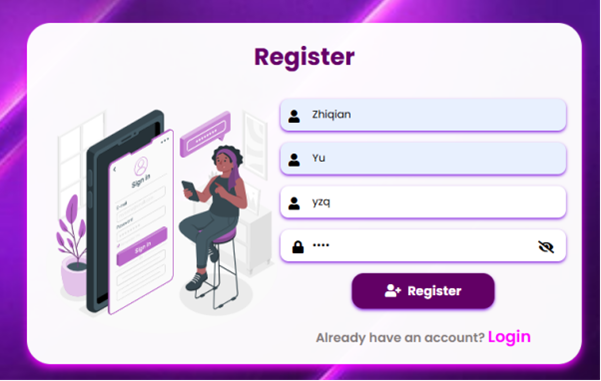
\includegraphics[width=\textwidth]{images/Demo_Registration.png}
        \caption*{(a) Demo Registration}
    \end{minipage}
    \hfill
    \begin{minipage}{0.5\textwidth}
        \centering
        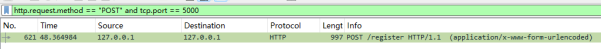
\includegraphics[width=\textwidth]{images/Capture_Information.png}
        \caption*{(b) Capture Information}
    \end{minipage}
    \hfill
    \begin{minipage}{0.5\textwidth}
        \centering
        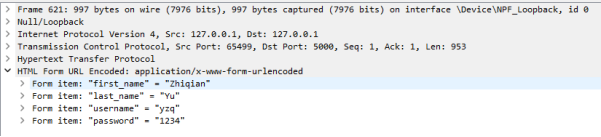
\includegraphics[width=\textwidth]{images/Information_content.png}
        \caption*{(c) Information content}
    \end{minipage}
    \hfill
    \begin{minipage}{0.5\textwidth}
        \centering
        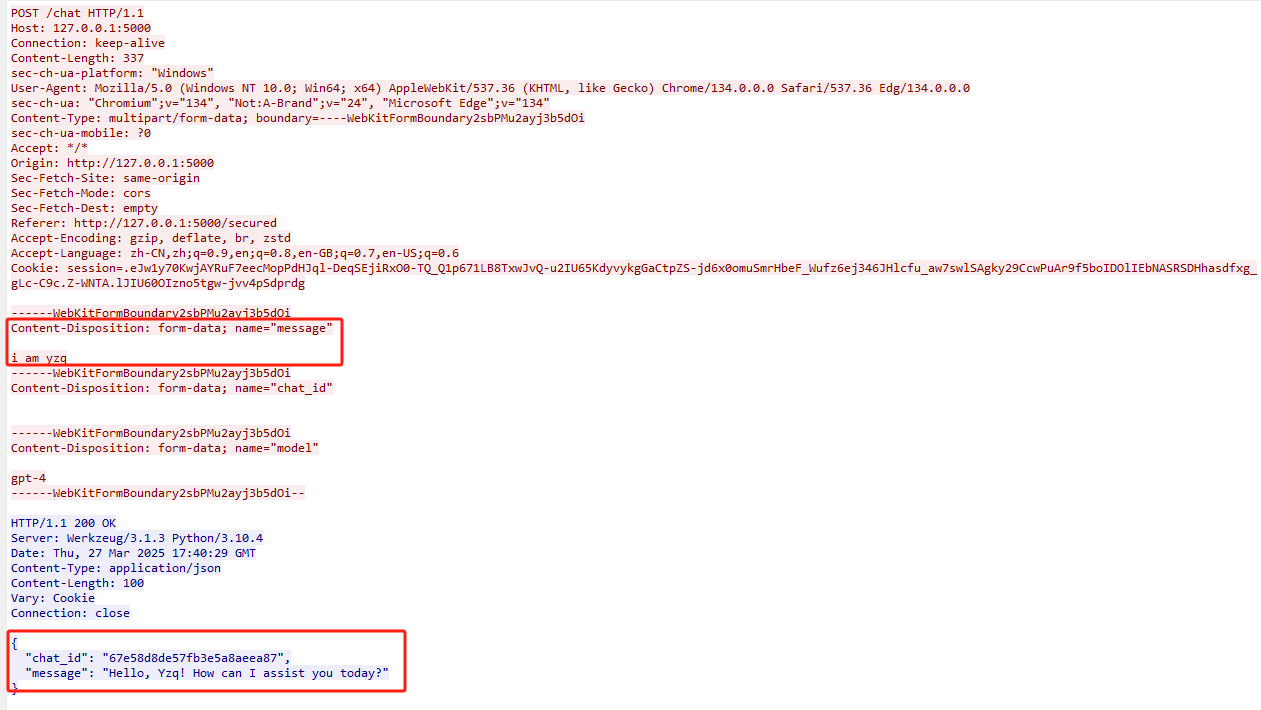
\includegraphics[width=\textwidth]{images/AI_dialogue_Information_content.png}
        \caption*{(d) AI dialogue Information content}
    \end{minipage}
    
    \caption{Wireshark's HTTP message capture}
    \label{fig:Demo Registration}
\end{figure}

\subsubsection{Session Hijacking}
After the user has successfully logged in, there is a legitimate session cookie in the browser, at this point we can use Wireshark to get the value of this cookie through a packet grabber, inject the cookie into our own browser, and then visit the /secured page. This will allow us to access the /secured page without logging in, thus obtaining the user's privacy directly. 
As shown in Fig. \ref{fig:cookie}, we have captured a login request in wireshark that contains a cookie message.

\begin{figure}[htb]
    \centering
    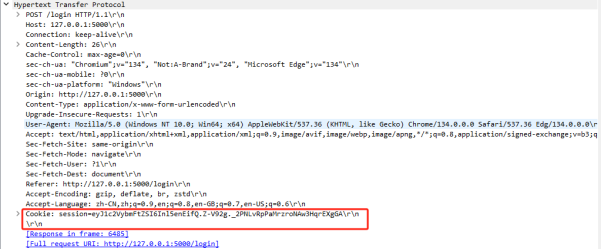
\includegraphics[width=0.5\textwidth]{images/Information_of_Cookie.png}
    \caption{Information of Cookie}
    \label{fig:cookie}
\end{figure}

After getting this cookie information, open the login screen and enter the information shown in Fig. \ref{fig:cookie} in the Console, we will see that the system has recognised the content of the cookie. 
So we enter the page we need to go to in the web port which is http://127.0.0.1:5000/secured and we can see that we have successfully jumped to the user interface.
\begin{figure}[htb]
    \begin{minipage}{0.5\textwidth}
        \centering
        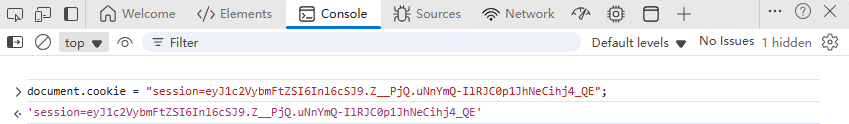
\includegraphics[width=\textwidth]{images/cookie_content.png}
        \caption*{(a) Cookie content}
    \end{minipage}
    \hfill
    \begin{minipage}{0.5\textwidth}
        \centering
        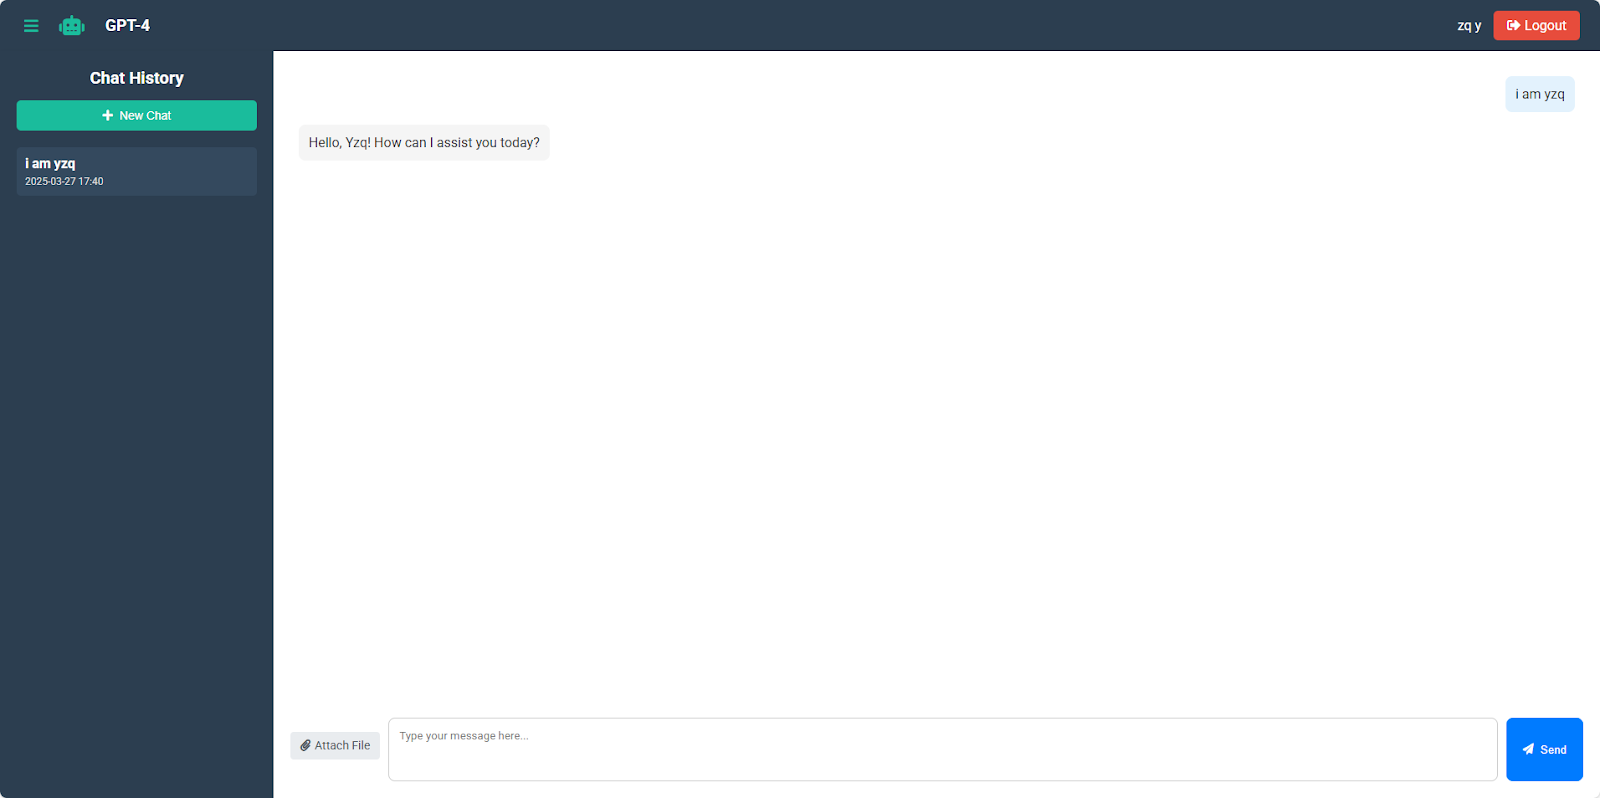
\includegraphics[width=\textwidth]{images/user_interface.png}
        \caption*{(b) User interface}
    \end{minipage}
    \caption{Information of Cookie}
    \label{fig:cookie}
\end{figure}

Applications allow users to log in with a username and password. In the original design, there was no rate limiting or CAPTCHA mechanism and the login endpoint was vulnerable to brute force attacks. We simulated an attacker using a multi-threaded Python script to systematically guess numeric passwords for known usernames. The script also allows the attacker to customize the length of the password to reduce the complexity of cracking if the user's account information is obtained by other means, such as the approximate length of the password or account name, etc. The script also allows the attacker to customize the length of the password to reduce the complexity of cracking. Once the correct password is recognized, the script terminates and saves the stolen credentials. For demonstration purposes, plain numbers are used as passwords and plain letters are used as user id.

\begin{figure}[htb]
    \centering
    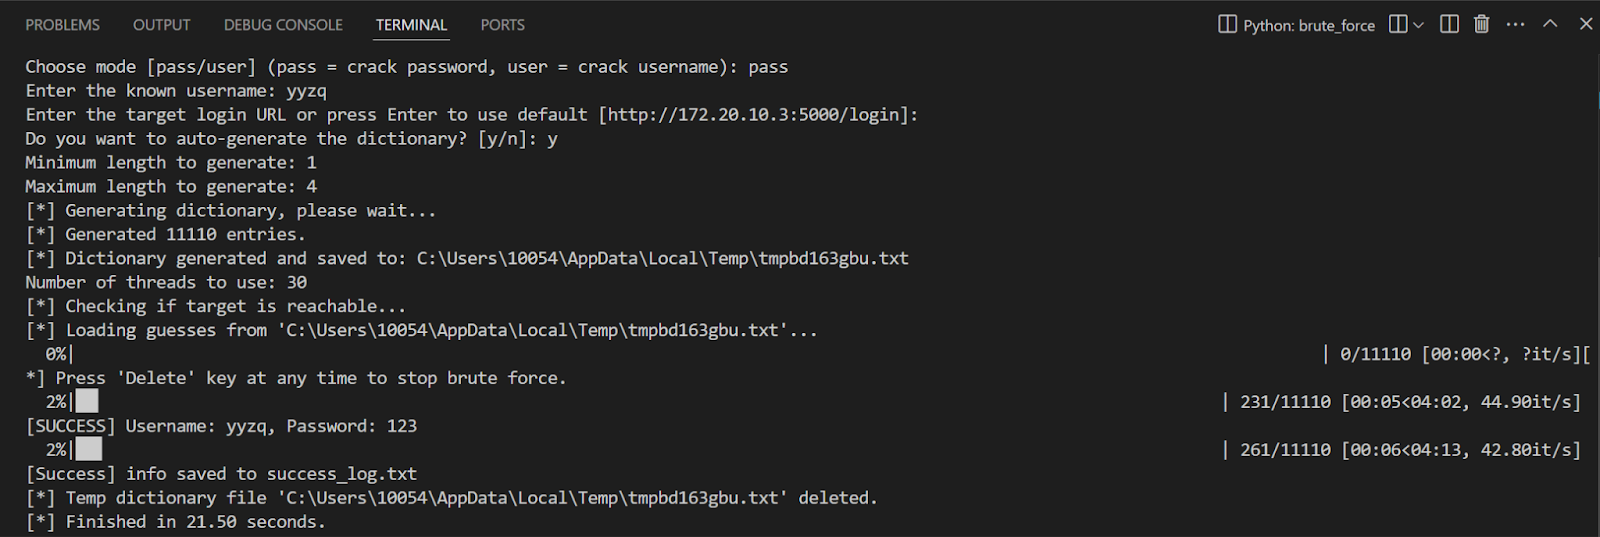
\includegraphics[width=0.5\textwidth]{images/Brute_force_attack_Python_script_demo.png}
    \caption{Brute force attack Python script demo}
    \label{fig:brute_force_attack}
\end{figure}

In addition, DDoS attacks are designed as decoys to cause confusion and create opportunities before executing attacks that actually threaten the security and privacy of user information. The initial Web services do not enforce any form of request limitation or IP blacklisting. An attacker can exhaust server resources by issuing a large number of seemingly legitimate HTTP GET requests. In the designed DDoS attack script, four types of attacks are included: HTTP Flood, UDP Flood, SYN Flood, and IP Fragment Flood.




% \vfill\pagebreak




\section{Coursework 2: Security \& Privacy Defense Strategy}
\subsection{Security (or Privacy or both) Interaction/visualisation/actuation system}
We propose a multi-layered, defense-in-depth architecture that integrates preventive, detective, and recovery mechanisms to mitigate the threats identified in our system.

For access control and authentication, we enforce Multi-Factor Authentication (MFA) using TOTP or device-based tokens and adopt a zero-trust architecture where each access request is continuously verified rather than implicitly trusted. User credentials are stored using bcrypt hashing to prevent SQL injection and accidental leaks by developers who can access the database. The rate limiting is also implemented to prevent brute-force attempts.

In terms of data security, all communication between client and server is secured via HTTPS, eliminating the risk of plain-text interception during login or session activity. Additionally, cookies are secured using flags such as HttpOnly, Secure, and SameSite=Strict to mitigate the risk of session hijacking through packet sniffing tools like Wireshark. To further ensure data integrity and legal compliance, we also implemented AI-driven content filtering that analyzes user input in real time. If violent, criminal, or otherwise illegal language is detected, the system will automatically block the content and prevent it from being written into the database. This preemptive measure helps us avoid storing unlawful data and enhances compliance with data protection regulations.

For backend integrity, we performed input validation to mitigate NoSQL injection attacks, ensuring user inputs are sanitized before being processed in MongoDB queries. We also implemented basic session binding, where a session is invalidated if the IP address does not match the original login IP, providing an extra layer of protection against session hijack scenarios.

These implementations significantly enhance the overall resilience of our system against practical threats such as interception, brute-force login, and injection-based exploits.

\subsection{Prototype Implementation and Demonstration}
This section illustrates the demonstration and implementation of the prototype we developed. This prototype demonstrates how real-world threats, such as plain text data transmission, unauthorized access, database breaches, and data pollution, can be mitigated using a layered security approach. The following subsections detail the practical setup and visual demonstration of these implementations, supported by code snippets, screenshots, and system behavior after applying each countermeasure.

\subsubsection{Enable TLS Encryption to Prevent Data Leakage }
First, because Wireshark may try to capture sensitive information (e.g. usernames, passwords, chats, etc.) in clear text, we implemented TLS encrypted communication for our web application, upgrading it from the original HTTP protocol to HTTPS, and this section documents the whole process from certificate generation to the Flask project's access to TLS. 
First, we generate a self-signed certificate and a private key locally using OpenSSL: cert.pem: server-side public key certificate and key.pem: private key. Then, in the Flask project, we enable TLS using the ssl\_context parameter, simply by specifying the path to cert.pem and key.pem at runtime. 
With this encryption, even if attackers use Wireshark to capture packets on the same network, they will not be able to obtain valid sensitive information. 
The data transmission process is changed from plain text to an encrypted stream, which significantly improves the security of user authentication, chat, and other operations.

\subsubsection{Add Email Verification Code as Double Authentication }
Next, we add the authentication scheme in the main interface, that is, we add the email verification code as a double guarantee, to prevent hackers from breaking in violently. 
To cooperate with the email authentication code function, we modify the specific requirements during registration. Besides the simple username and password, we add the registration of additional email information. 
The specific information is shown in the Fig. \ref{fig:email_verification} below.
\begin{figure}[htb]
    \begin{minipage}{0.5\textwidth}
        \centering
        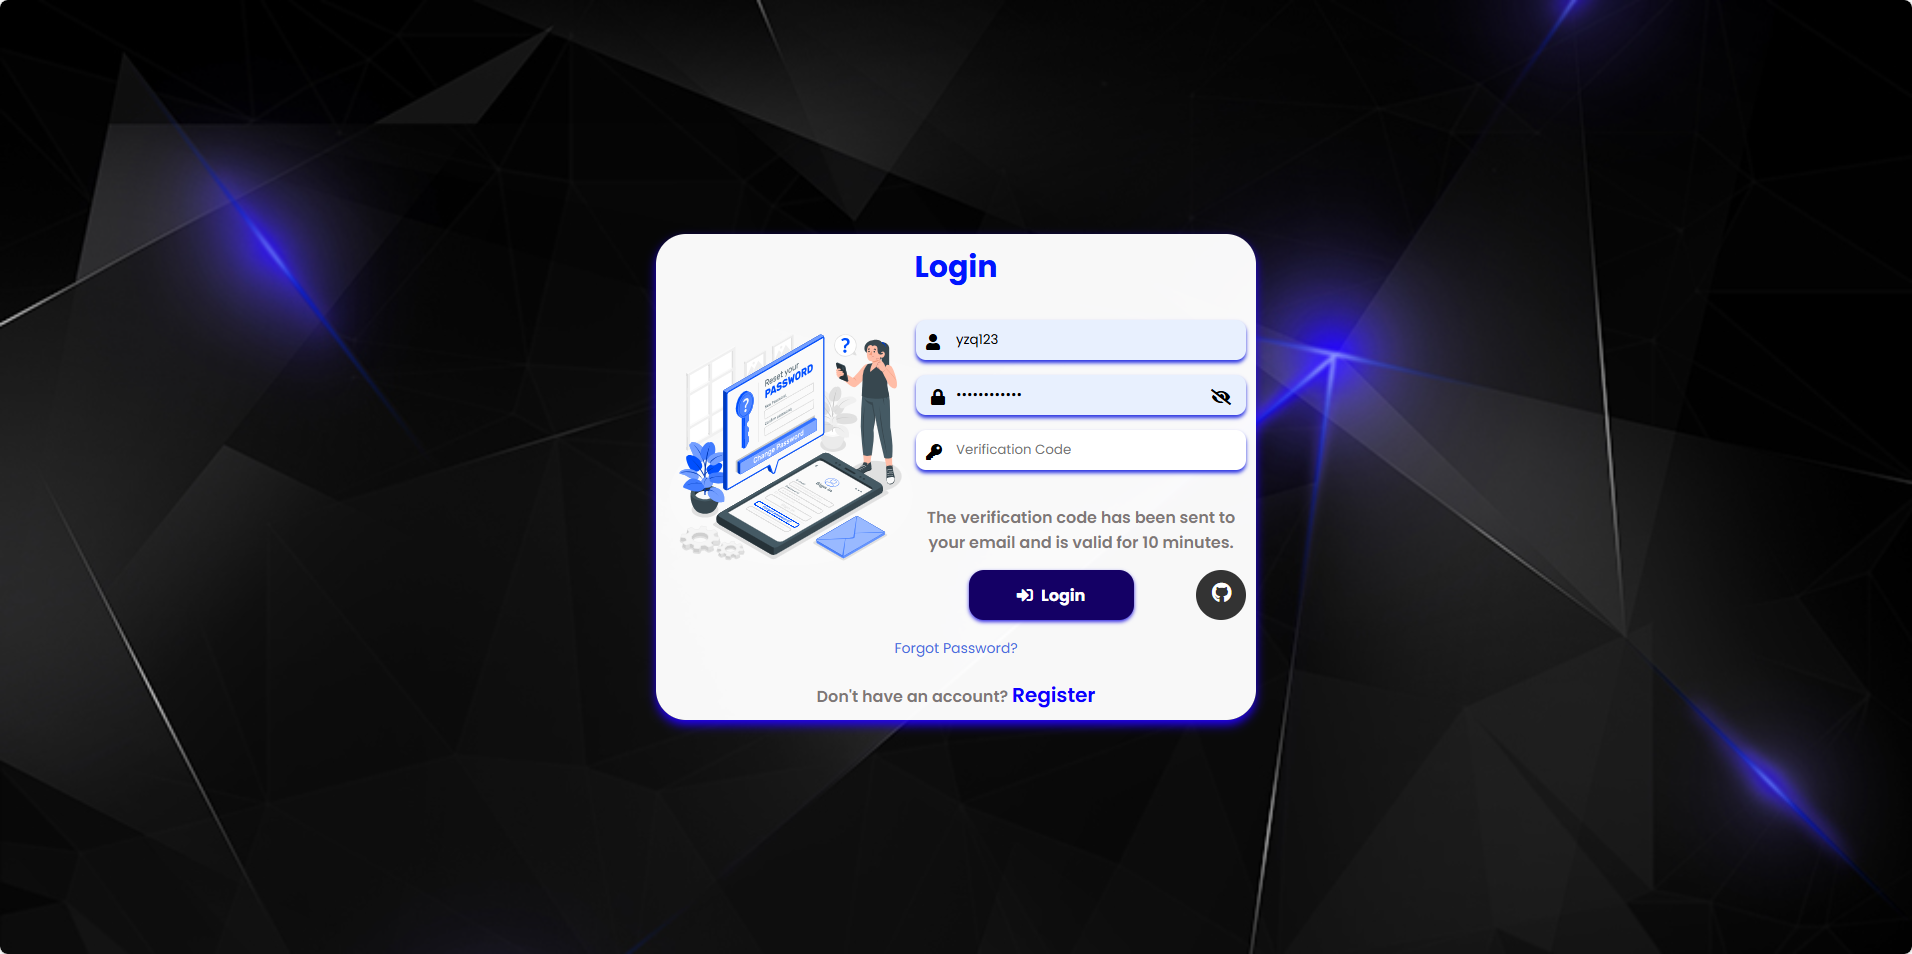
\includegraphics[width=\textwidth]{images/email_authentication_login_screen.png}
        \caption*{(a) Email verification login page}
    \end{minipage}
    \hfill
    \begin{minipage}{0.5\textwidth}
        \centering
 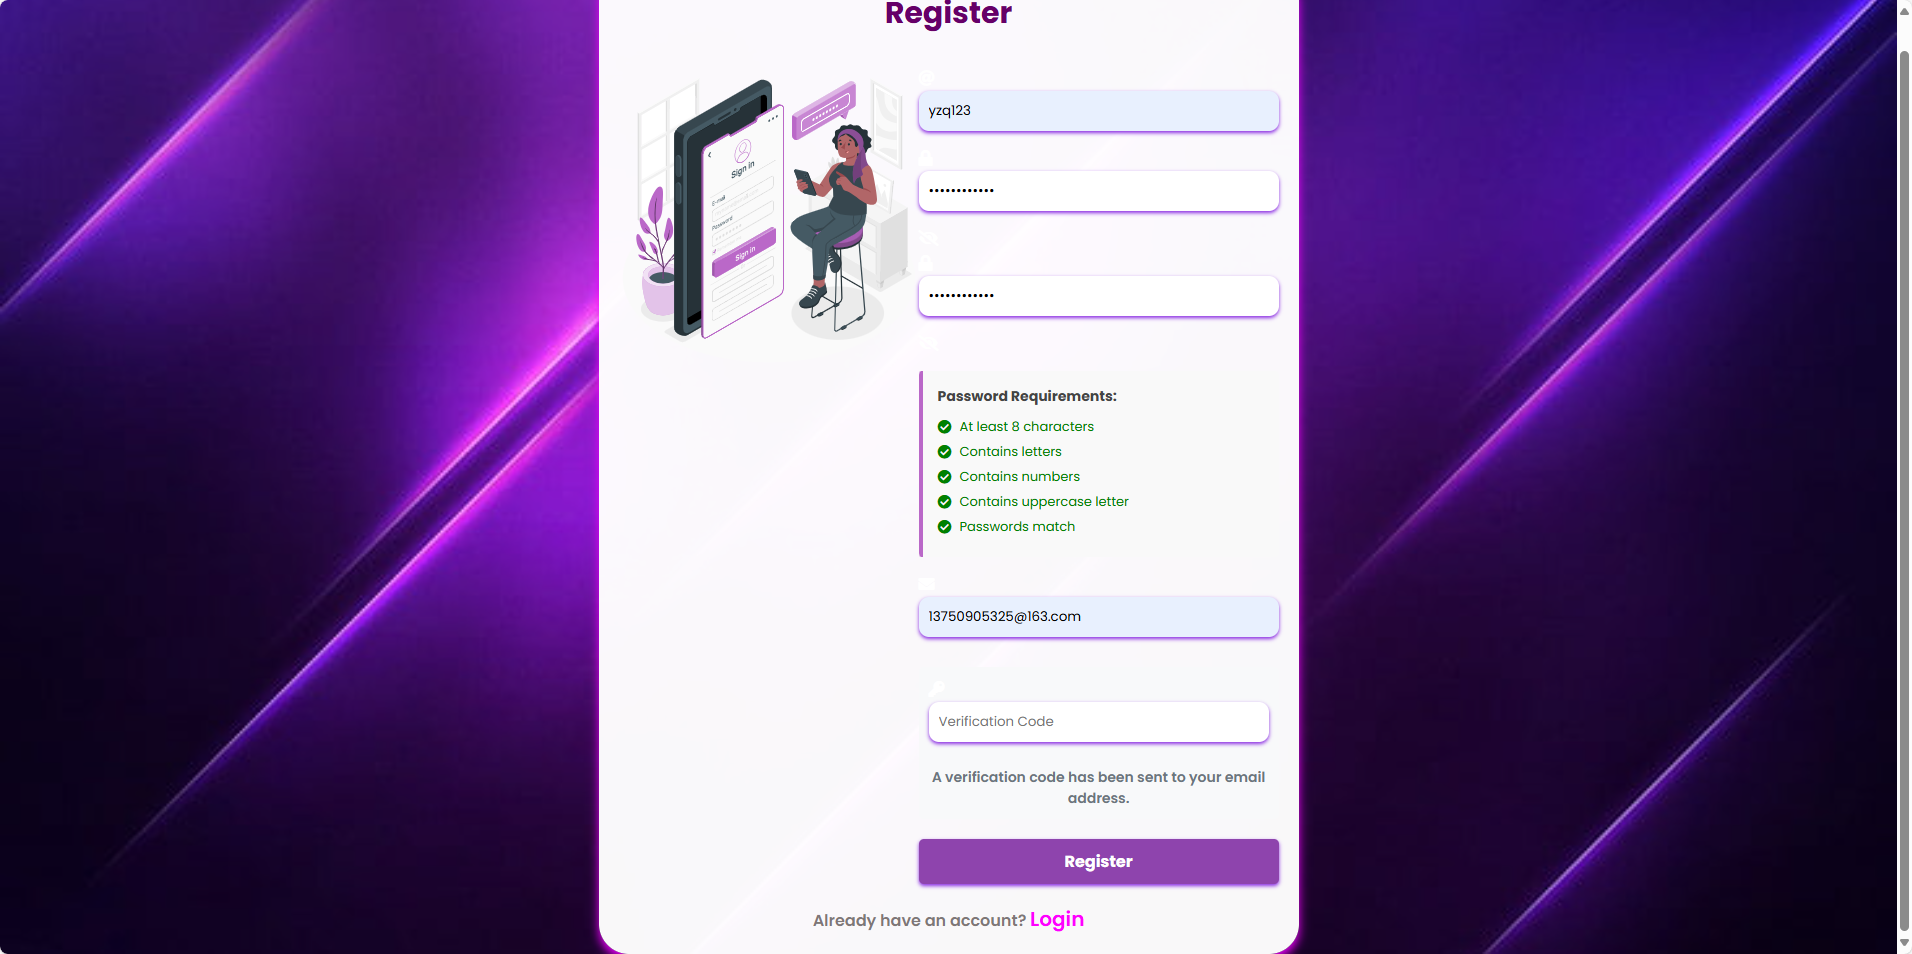
\includegraphics[width=\textwidth]{images/email_authentication_register_screen.png}
        \caption*{(b) Email verification registration page}
    \end{minipage}
    \caption{Email verification}
    \label{fig:email_verification}
\end{figure}

\subsubsection{Encrypt Sensitive Information in the Database }
At the same time we are registering information into the database, considering the use of the MongoDB database itself has a very strong privacy protection mechanism, so we do not consider for the time being the processing of this database. 
But in this particular case, after grabbing the .env file, we also have the opportunity to enter the database through the URI. 
Therefore, when we store the relevant information, as shown in the Fig. \ref{fig:hash} below, we encrypt the password with a hash algorithm, which can effectively protect the user's information even if it is illegally invaded.
\begin{figure}[htb]
    \centering
    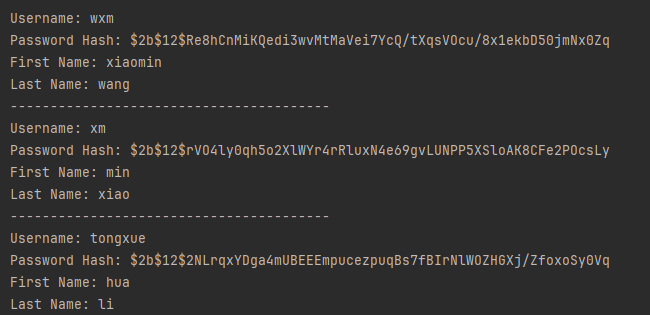
\includegraphics[width=0.5\textwidth]{images/Partially_encrypted_information.png}
    \caption{Partially encrypted information}
    \label{fig:hash}
\end{figure}
\subsubsection{AI-based Mechanism to Prevent Sensitive Data Pollution }
To implement an effective mechanism for detecting and filtering sensitive or toxic user input to prevent them from entering the database and polluting the content, we developed a lightweight text classification model capable of distinguishing between safe and harmful content. The model was trained using a labeled dataset containing example sentences that were manually categorized as either benign or containing inappropriate language, such as violent, abusive, or otherwise prohibited expressions. 

\subsubsection{Train Dataset}
The train dataset is from the Toxic Comment Classification Challenge on Kaggle\footnote{https://www.kaggle.com/c/jigsaw-toxic-comment-classification-challenge/data?select=train.csv.zip}. The dataset consists of approximately 160,000 text samples, each annotated with six binary labels indicating different types of harmful content: toxic, severe\_toxic, obscene, threat, insult, and identity\_hate. Each label is represented as either 0 or 1, signifying the absence or presence of the respective trait in the text. To simplify the classification task into a binary setting, we consolidated these six labels into a single unified label. Specifically, if a sample is marked with a value of 1 in any of the six categories, we consider it harmful and assign it a final label of 1; otherwise, the label is 0. This preprocessing step allows the model to focus on general toxic language detection rather than distinguishing between different subtypes of harmful content, which is more suitable for our goal of preventing any sensitive or offensive text from entering the database. 

\subsubsection{Model}
The model used is a pre-trained Bert-base-uncase model\footnote{https://huggingface.co/google-bert/bert-base-uncased } \cite{devlin2018bert}. It consists of 12 transformer layers (also called encoder blocks), 768 hidden units per layer, and 12 attention heads, totaling approximately 110 million parameters. As a deep bidirectional model, it considers both left and right context in all layers, making it highly effective for capturing the meaning and nuances of natural language. By using this model as a feature extractor or fine-tuning it for binary classification, we are able to significantly improve the model’s ability to detect toxic and sensitive content.

\subsubsection{Result}
Due to the large size of the training dataset and the limitations of available computational resources, we limited the model training to 3 epochs. During training, the model parameters were updated using the Adam optimizer with weight decay, and binary cross-entropy was used as the loss function.  Table 1 shows the model performance over epochs. The model achieved over 96\% accuracy, with F1 scores remained stable, suggesting that the model had learned meaningful patterns without significant overfitting. 
\begin{table}
\centering
\caption{Model performance over epochs}
\begin{tabular}{|c|c|c|c|}
\hline
\textbf{Epoch} & \textbf{Training Loss} & \textbf{Accuracy} & \textbf{F1 Score} \\
\hline
1 & 0.182700 & 0.955500 & 0.820721 \\
2 & 0.072100 & 0.960000 & 0.817352 \\
3 & 0.021700 & 0.960500 & 0.819222 \\
\hline
\end{tabular}
\label{tab:training_metrics}
\end{table}

After training, the model was uploaded to the Hugging Face Model Hub \footnote{https://huggingface.co/ZheZHEZHE020106/zt-harmful_language_detecting}, which allows the model to be directly loaded via the transformers library without any additional configuration. Finally, we integrated it into the Flask backend.

As shown in the Fig. \ref{fig:pollution}, although we present four dialogues in the dialogue box, the AI system detects that some of the dialogues contain sensitive words and therefore initiates a warning. 
And we can also clearly see in the database that the content stored in the database does not contain the sensitive content that was warned.

\begin{figure}[H]
    \begin{minipage}{0.5\textwidth}
        \centering
        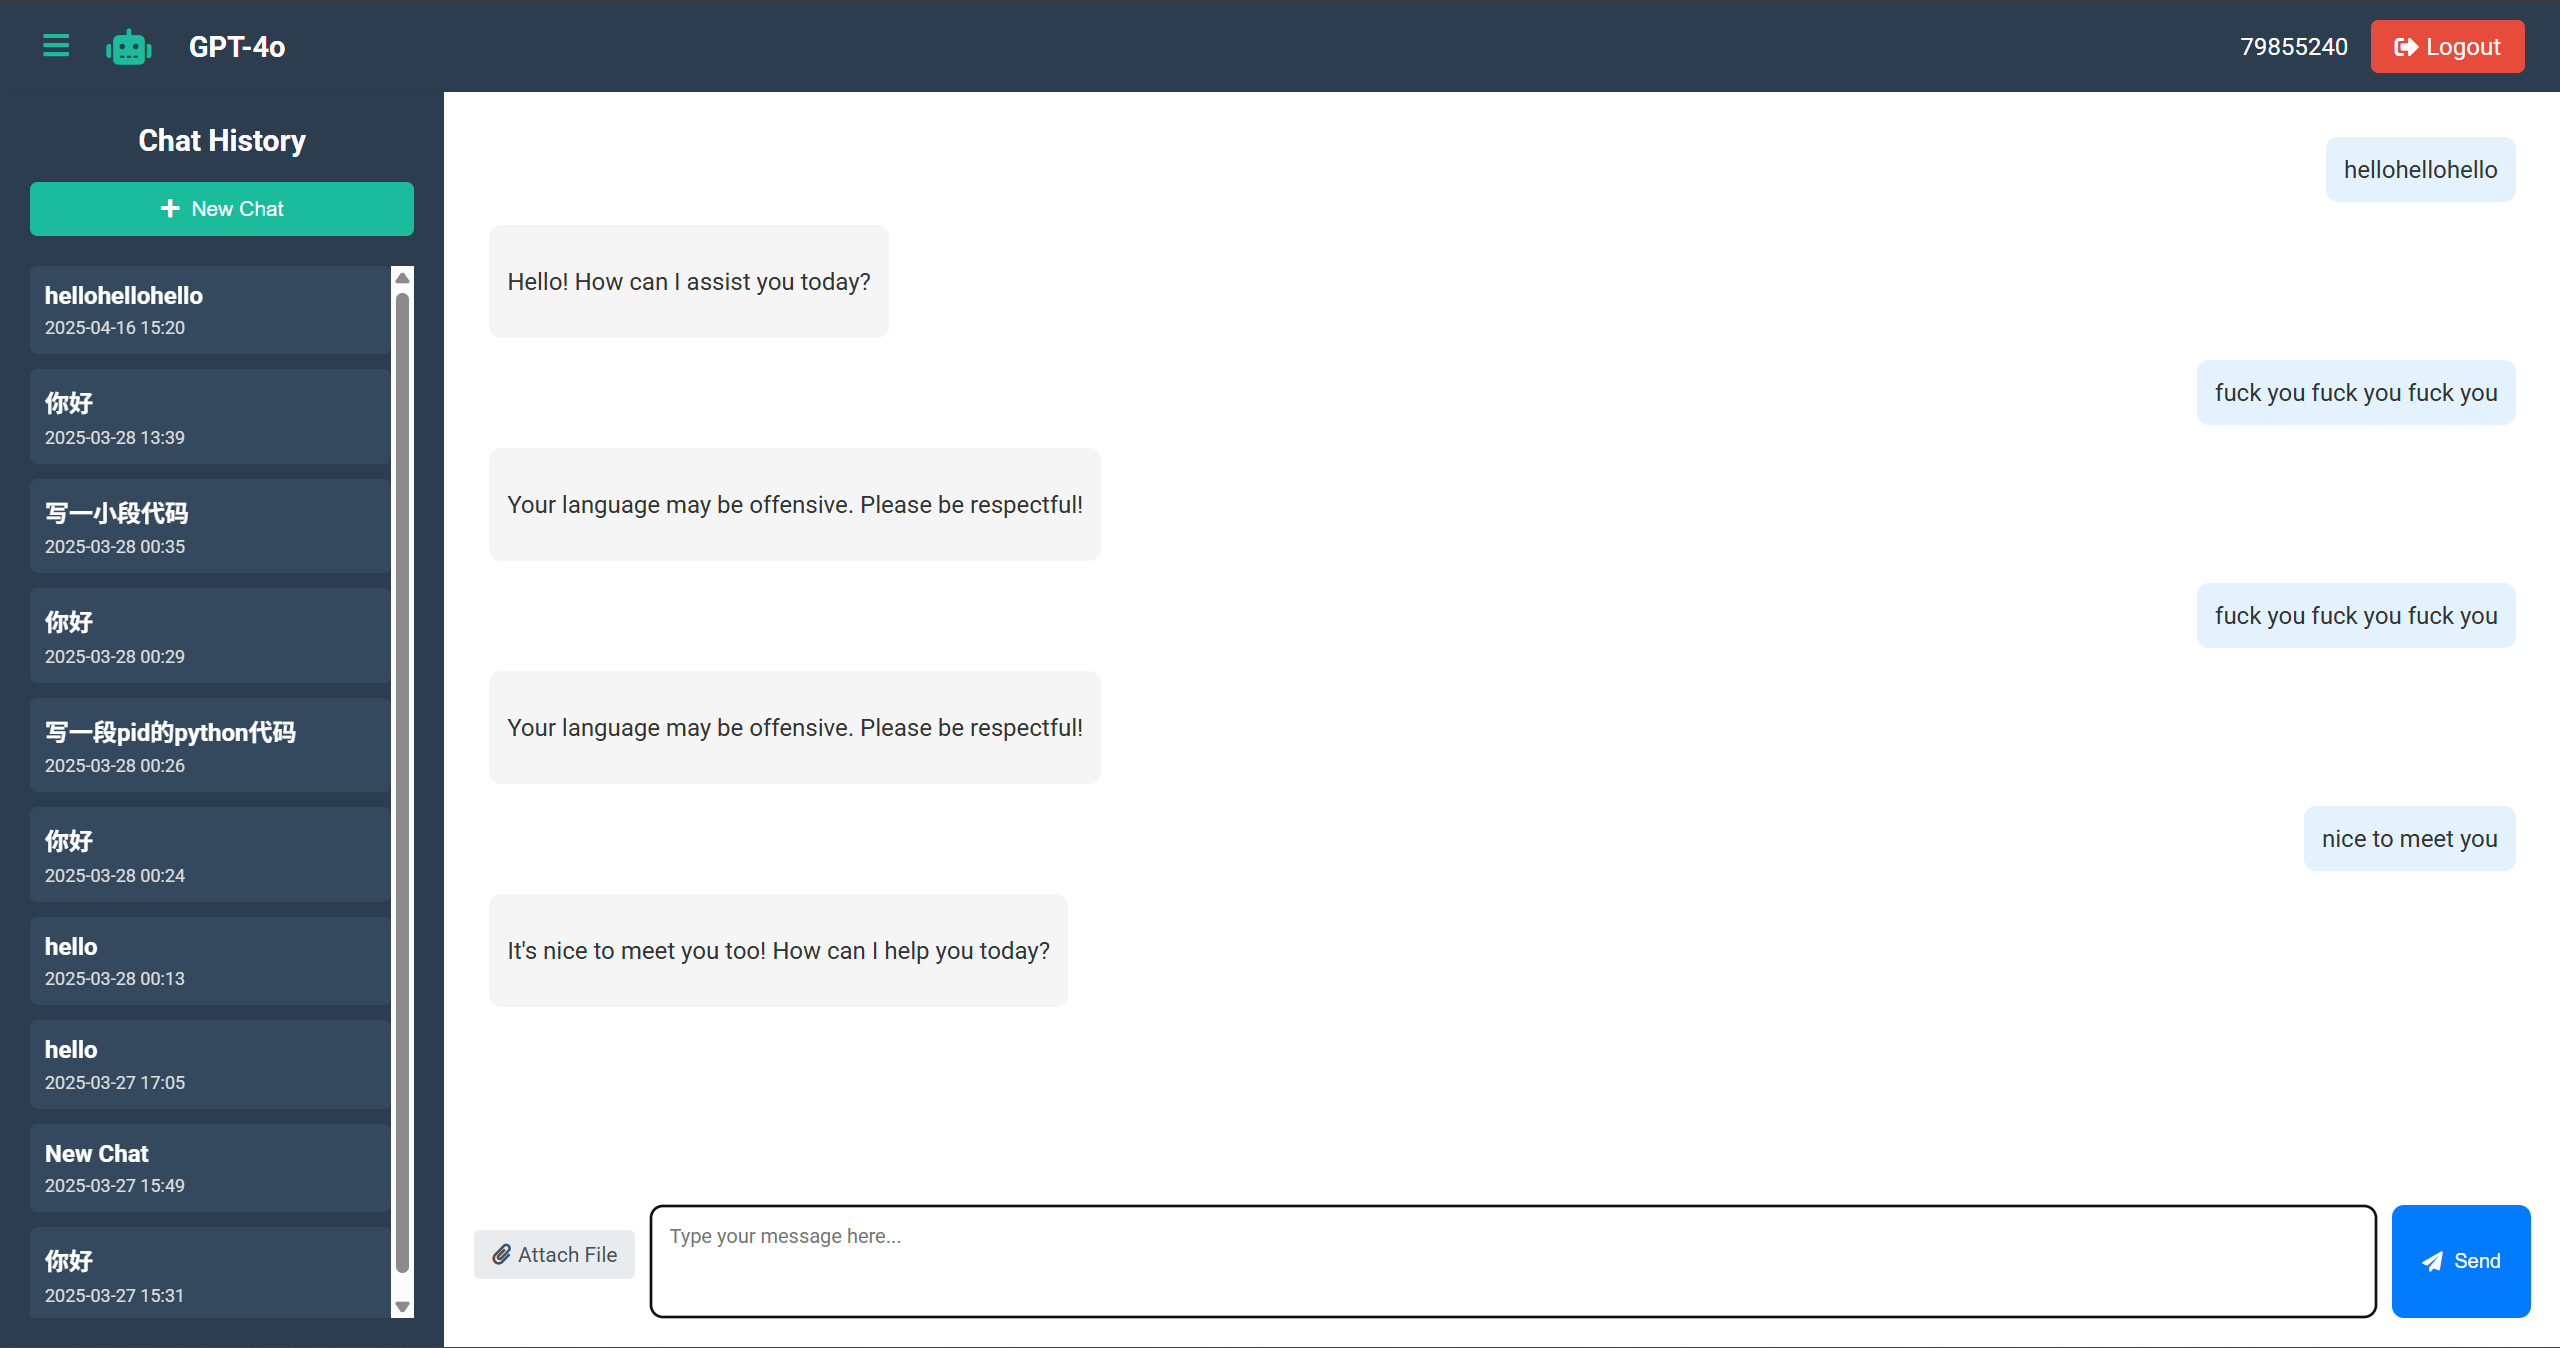
\includegraphics[width=\textwidth]{images/Chat_interface_after_anti_pollution.png}
        \caption*{(a) Chat interface after anti-pollution}
    \end{minipage}
    \hfill
    \begin{minipage}{0.5\textwidth}
        \centering
        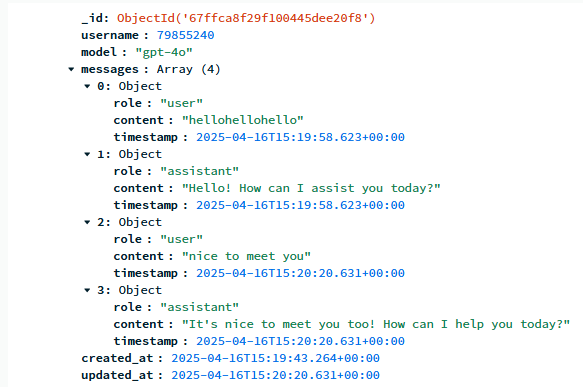
\includegraphics[width=\textwidth]{images/Database_information_after_anti_pollution.png}
        \caption*{(b) Database information after anti-pollution}
    \end{minipage}
    \caption{AI dialogue system after anti-pollution}
    \label{fig:pollution}
\end{figure}


\subsection{Regulation and Ethical considerations}

Our system's security architecture must comply with major data protection and cybersecurity regulations while addressing critical ethical considerations around AI implementation.

\subsubsection{Regulatory Compliance}

The system has been designed to meet requirements from three key regulatory frameworks:

\textbf{General Data Protection Regulation (GDPR):}

\begin{itemize}
    \item Personal data protection is implemented through bcrypt password hashing, secure MongoDB storage patterns, and Flask session management
    \item User consent and control mechanisms include time-limited verification codes and email validation for authentication events
    \item Data minimization principles are followed by collecting only essential information for functionality
\end{itemize}

\textbf{Cyber Resilience Act (CRA):}

\begin{itemize}
    \item Security-by-design principles implemented through comprehensive input validation and anti-brute force mechanisms with account lockouts
    \item Vulnerability handling through multi-factor authentication and AI-driven content filtering
    \item Regular security audits are performed to identify potential weaknesses
\end{itemize}

\textbf{Product Security and Telecommunications Infrastructure Act (PSTI):}

\begin{itemize}
    \item Secure communication through HTTPS/TLS implementation and encrypted authentication tokens
    \item Data security in transit and storage via validated file upload handling and secure binary storage
\end{itemize}

\subsubsection{Ethical Considerations}

Several ethical challenges were identified and addressed:

\textbf{Surveillance and Privacy Risks:}

\begin{itemize}
    \item Implemented data retention policies with automatic anonymization for older conversations
    \item Added transparent user controls for data management
    \item Created clear privacy notices explaining data collection practices
\end{itemize}

\textbf{User Consent:}

\begin{itemize}
    \item Added explicit consent checkboxes during registration for data processing
    \item Implemented a user data dashboard for visibility and control
    \item Established straightforward processes for data deletion requests
\end{itemize}

\textbf{AI-Driven Security Concerns:}

\begin{itemize}
    \item Created an appeals process for content moderation decisions
    \item Regular auditing of toxicity detection models for bias
    \item Transparent disclosure of AI processing to users
\end{itemize}

\textbf{Security vs. Usability Balance:}

\begin{itemize}
    \item Provided clear guidance on security requirements
    \item Implemented progressive security based on operation sensitivity
    \item Offered alternative authentication methods for accessibility
\end{itemize}

The system achieves a balance between robust security and ethical responsibility, ensuring both compliance with regulatory requirements and respect for user privacy and autonomy. These considerations are particularly important in AI systems where automated decisions impact user experience and data handling.



\subsection{Scalability, Innovation \& Enterprise Considerations}

Here's the content for your Scalability, Innovation \& Enterprise Considerations section:

\subsection{Scalability, Innovation \& Enterprise Considerations}

\subsubsection{Enterprise Scalability}
To ensure our system scales effectively for enterprise adoption, we propose a multi-layered approach to infrastructure development. For technical infrastructure, containerization through Docker and orchestration via Kubernetes would allow horizontal scaling based on demand and consistent deployment across environments. Our MongoDB implementation would evolve to incorporate sharding for distributed storage, replica sets for high availability, and connection pooling to handle thousands of concurrent users.

Performance at scale would be achieved through strategic implementation of Redis or Memcached for session management, response caching for frequent AI queries, CDN integration, and appropriate API rate limiting. This infrastructure would support essential enterprise authentication integration requirements, including:

\begin{itemize}
    \item SAML for Single Sign-On integration
    \item LDAP/Active Directory for enterprise user management
    \item Expanded OAuth provider support
    \item Advanced MFA protocols for organizational security policies
\end{itemize}

For operational stability at scale, we would implement comprehensive monitoring through an ELK stack or similar solution, real-time metrics with Prometheus/Grafana, custom health dashboards, and automated alerting for system issues. Additionally, CI/CD pipelines would ensure reliable deployment with automated testing, canary deployments, and infrastructure-as-code practices.

\subsubsection{Innovative Security Approaches}
Our platform implements several innovative approaches that differentiate it from traditional security methods:

\textbf{Contextual Authentication:} Beyond our current MFA system with time-limited verification codes, we propose implementing adaptive authentication that adjusts security requirements based on risk factors including login location, device profile, and established activity patterns.

\textbf{AI-Powered Content Security:} Our existing ML-based content moderation can be extended to detect potential security threats such as social engineering attempts and data exfiltration in user prompts, creating an intelligent defensive layer that evolves with threats.

\textbf{Privacy-Preserving AI:} We propose implementing federated learning techniques to improve AI security models without exposing sensitive user conversation data, and exploring homomorphic encryption to allow AI processing on encrypted data while maintaining privacy.

\textbf{Zero-Trust Architecture:} Unlike traditional perimeter-based security, our design validates every request and could implement continuous validation throughout user sessions with real-time permission adjustments based on behavioral patterns.

\subsubsection{Long-term Viability and Cost Management}
The long-term sustainability of our security architecture depends on balanced resource allocation and strategic planning. For cost optimization, we would implement:

\begin{itemize}
    \item Tiered usage plans based on organizational needs
    \item Automatic scaling during varying usage periods
    \item Token/query budgeting with department-specific tracking
    \item Advanced caching strategies to reduce redundant AI calls
\end{itemize}

Future-proofing strategies include designing for quantum resistance by implementing post-quantum cryptographic algorithms where possible, establishing a component replacement strategy for rapid integration of emerging security technologies, and maintaining compliance flexibility through modular policy engines that adapt to regulatory changes.

Through these comprehensive approaches to scalability, innovation, and long-term planning, our platform can evolve from a demonstration project into an enterprise-ready system capable of supporting thousands of users while maintaining security, performance, and regulatory compliance.


\vfill\pagebreak

% References should be produced using the bibtex program from suitable
% BiBTeX files (here: strings, refs, manuals). The IEEEbib.bst bibliography
% style file from IEEE produces unsorted bibliography list.
% -------------------------------------------------------------------------
\bibliographystyle{IEEEbib}
\bibliography{refs}




\end{document}
